%% Los cap'itulos inician con \chapter{T'itulo}, estos aparecen numerados y
%% se incluyen en el 'indice general.
%%
%% Recuerda que aqu'i ya puedes escribir acentos como: 'a, 'e, 'i, etc.
%% La letra n con tilde es: 'n.

\chapter*{Propuesta y Justificaci\'on}
\addcontentsline{toc}{chapter}{Propuesta y Justificaci\'on}

Debido a la atenci'on que se tiene en la tecnolog'ia en la nube, los centros de datos han tomado un papel muy importante para los servicios empresariales.\cite{shimpy2014different} Un centro de datos est'a compuesto por miles servidores virtuales ejecut'andose en una instancia de tiempo, alojando muchas tareas al mismo tiempo el centro de datos recibe miles de peticiones a esas tareas. Es aqu'i en donde la programaci'on de tareas tiene un rol demasiado importante para el c'omputo en la nube porque influye en el rendimiento del mismo.\cite{srinivasan2014cloud} 

El problema de la calendarizaci'on pertenece a los algoritmos NP-Dif'icil, lo cual tiene un amplio rango de soluciones posibles y se toma mucho m'as tiempo de encontrar una respuesta 'optima ya que no existe un m'etodo para resolver estas inc'ognitas. Sin embargo es posible estar cerca de la mejor soluci'on contemplando algunos entornos.\cite{shimpy2014different}

En esta investigaci'on se propondr'a una mejora a un algoritmo de calendarizaci'on para el caso de estudio de un sistema ERP en la nube, contemplando sus posibles escenarios y peticiones heterog'eneas. De esta manera se podr'a contar con un esquema de distribuci'on de trabajos que satisfaga las necesidades de un sistema ERP, mejorando el tiempo de respuesta y aprovechando los recursos. Con beneficios a los proveedores de servicios(SaaS) de sistemas ERP.

\begin{figure}
	
	\centering
	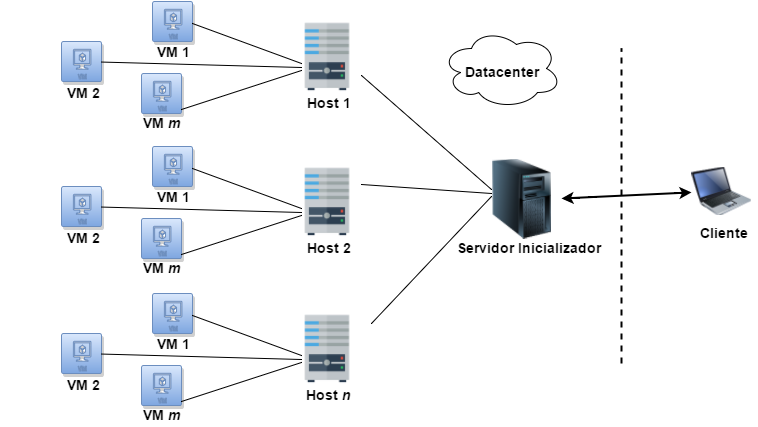
\includegraphics[scale=0.5]{media/cloud2}
	\caption{Propuesta de arquitectura en la nube}
\end{figure}
%%%%%%%%
%%  IMAGEN
%%%


En la figura 2 se puede observar la arquitectura del centro de datos que se implementar'a en la investigaci'on, el cual est'a compuesto de los siguientes elementos:

\begin{itemize}
\item \textbf{Servidor administrador:} Es el servidor que tendr'a el rol de front end en el centro de datos, teniendo una interacci'on directa con las peticiones de los usuarios, que son especificados en 'este documento como trabajos.
El principal objetivo de 'este elemento es delegar los trabajos a las m'aquinas virtuales en los distintos hosts del centro de datos.
\item \textbf{Host:} es el recurso de hardware que se tiene en el centro de datos. Una de las caracter'isticas de 'este elemento es que es finito.
\item \textbf{M'aquinas Virtuales:} son instancias dentro de los host, tienen como objetivo resolver los trabajos que se les sea asignado.


\end{itemize}